\documentclass{article}

\usepackage[english, russian]{babel}
\usepackage{amsmath}
\newcommand{\Mod}[1]{\ (\mathrm{mod}\ #1)}
\usepackage[letterpaper,top=2cm,bottom=2cm,left=3cm,right=3cm,marginparwidth=1.75cm]{geometry}
\usepackage[usenames,dvipsnames]{color}

\setlength{\abovedisplayskip}{3pt}
\setlength{\abovedisplayshortskip}{3pt}
\setlength{\belowdisplayskip}{3pt}
\setlength{\belowdisplayshortskip}{3pt}
\usepackage[14pt]{extsizes} 

\DeclareMathAlphabet{\pazocal}{OMS}{zplm}{m}{n}
\newcommand{\unif}{\pazocal{U}}

\linespread{1.6}

\usepackage{amsmath}
\usepackage{graphicx}
\usepackage[colorlinks=true, allcolors=blue]{hyperref}
\usepackage{fancyvrb} % for "\Verb" macro
\VerbatimFootnotes    % enable use of \Verb in footnotes

\title{Краткое описание решения.}
\date{}
\begin{document}
\maketitle

Основные работы на которые я опирался указаны в \href{https://github.com/koshachya-myata/RL_DataCener_Literature}{репозитории}, а также в прошлых отчетах.


\section{Построение модели ЦОД}
В данной секции описан процесс построения модели ЦОД.

\subsection{Общее описание модели}
Модель ЦОД создавалась с использованием OpenStudio и EnergyPlus. Сама модель описывается в файле формата \Verb+.idf+, с помощью специального языка разметки, этот файл подается в EnergyPlus для запуска процесса моделирования. Также использовалось приложение OpenStudio Application, которое позволяет сделать некоторую часть работы с помощью приложения с графическим интерфейсом. Некоторые рисунки ниже это скриншоты из этого приложения.

ЦОД состоит из помещения 31x4x18 метров. Используемые материалы и конструкции подбирались под климатическую зону 6A (ASHRAE CLIMATE ZONE). Помещение разделено на 11 температурных зон. Первая зона – горячая, далее типы зон чередуются. Для горячих зон установлена нагрузка 1000 Вт/м\textsuperscript{2} (исключение -- первая и последняя горячие зоны, для них установлено значение в 500 Вт/м\textsuperscript{2}). Для холодных зон нагрузка отсутствует (за исключением минимальной осветительной нагрузки). Между зонами стоит воздушная стена (air boundary construction), через нее зоны могут обмениваться воздухом (и соответственно температурой). Ширина холодных коридоров – 2 метра. Крайних горячих – 3 метра, промежуточных – 4 метра.

Под основным помещением установлен фальшпол. Внутри ЦОД стоит система CRAH, которая ориентируется на температуру внутри холодных зон. Холодный воздух подается внутрь фальшпола под управлением системы CRAH, а затем из фальшпола холодный воздух попадает в холодные коридоры.
Модель здания представлена на Рис. \ref{fig:DC_model}.

\begin{figure}[h!]
\centering
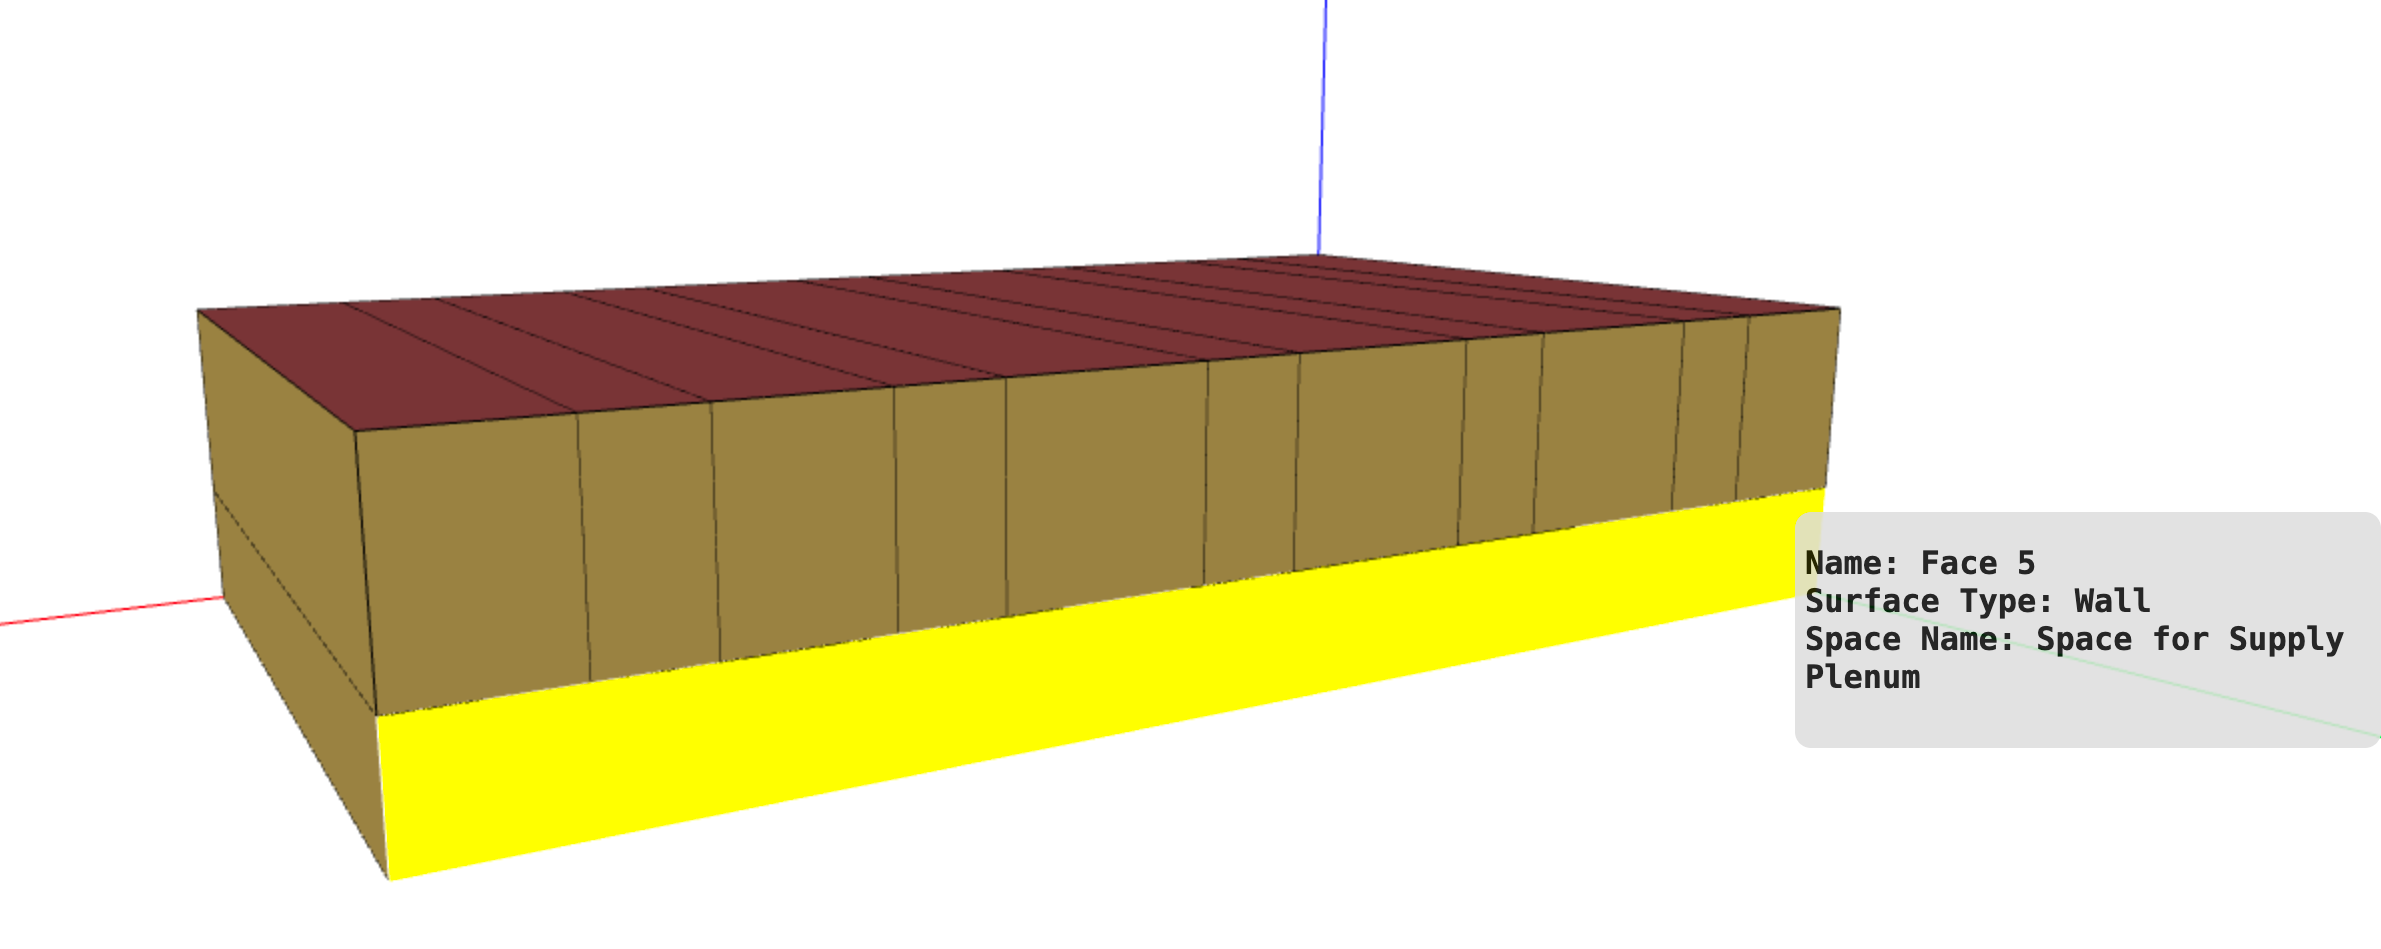
\includegraphics[width=0.8\linewidth]{figures/DC_model.png}
\caption{Модель здания ЦОД.}
\label{fig:DC_model}
\end{figure}

Для каждой поверхности указан ее тип, а для каждого типа установлена конструкция (состоящая из слоев материалов), из которой эта поверхность состоит (Рис. \ref{fig:DC_constructions})

\begin{figure}[h!]
\centering
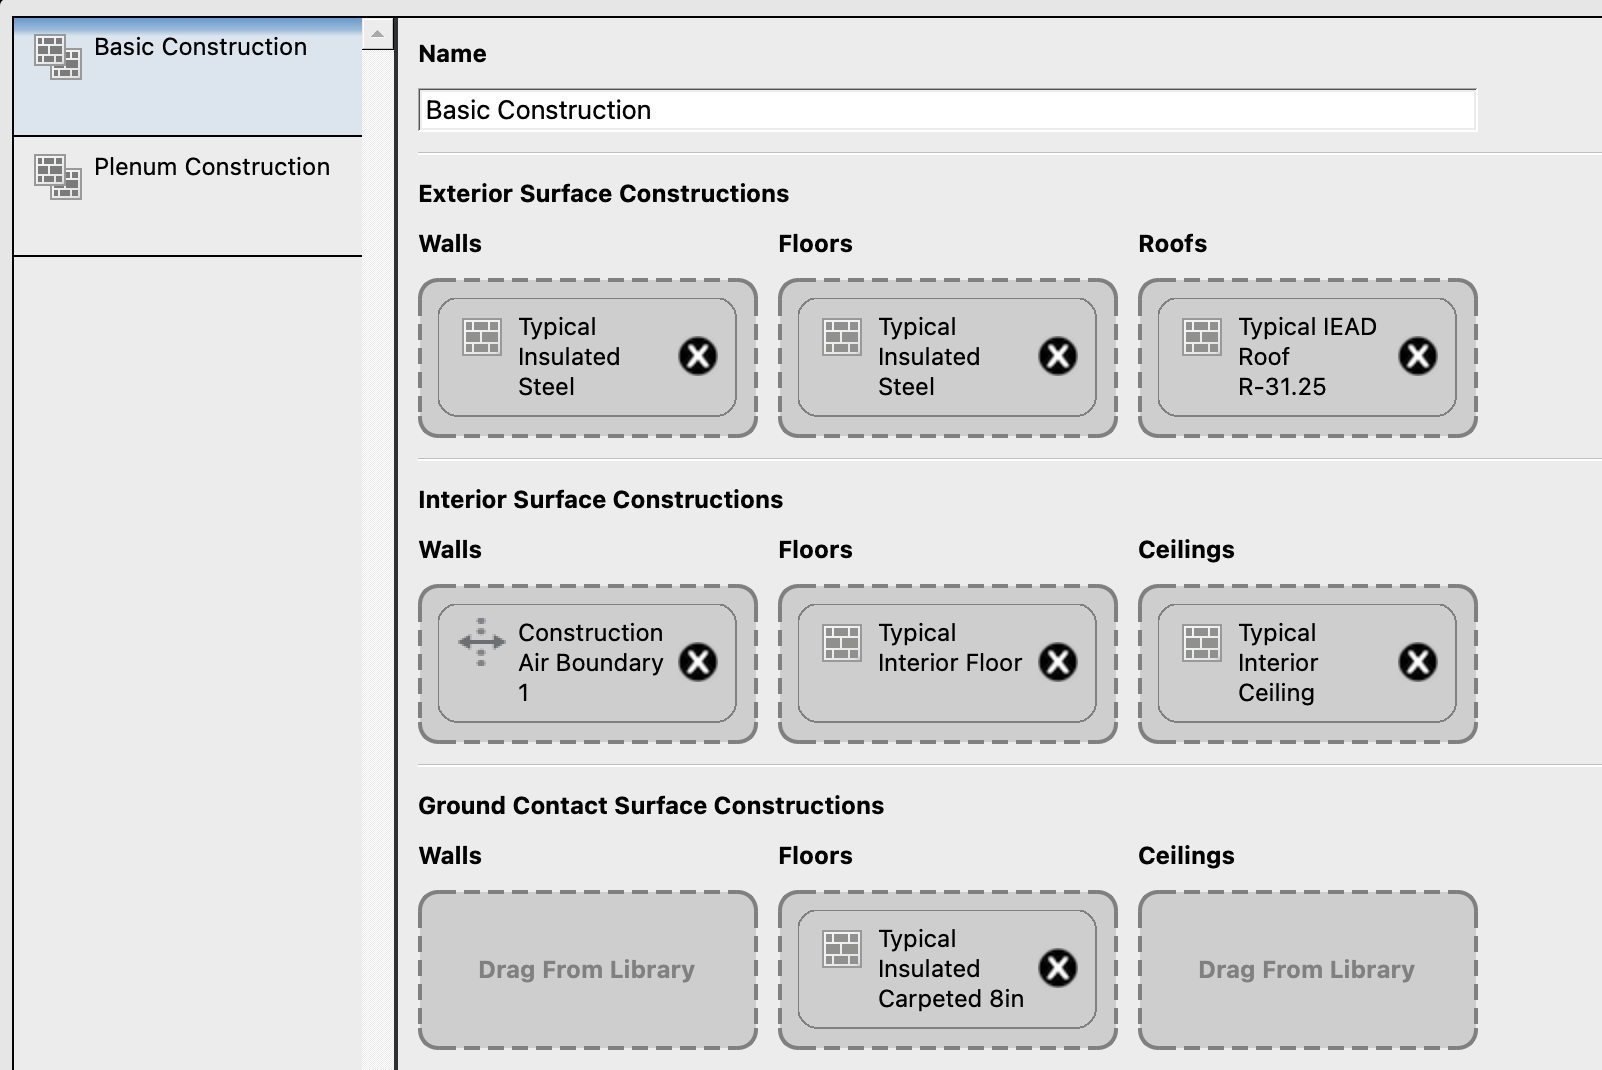
\includegraphics[width=0.8\linewidth]{figures/DC_constructions.png}
\caption{Конструкции основного помещения модели ЦОД.}
\label{fig:DC_constructions}
\end{figure}

Визуализация очередности холодных коридоров внутри здания представлена на Рис. \ref{fig:aisles_zones}. Между холодными коридорами расположены горячие. 

\begin{figure}[h!]
\centering
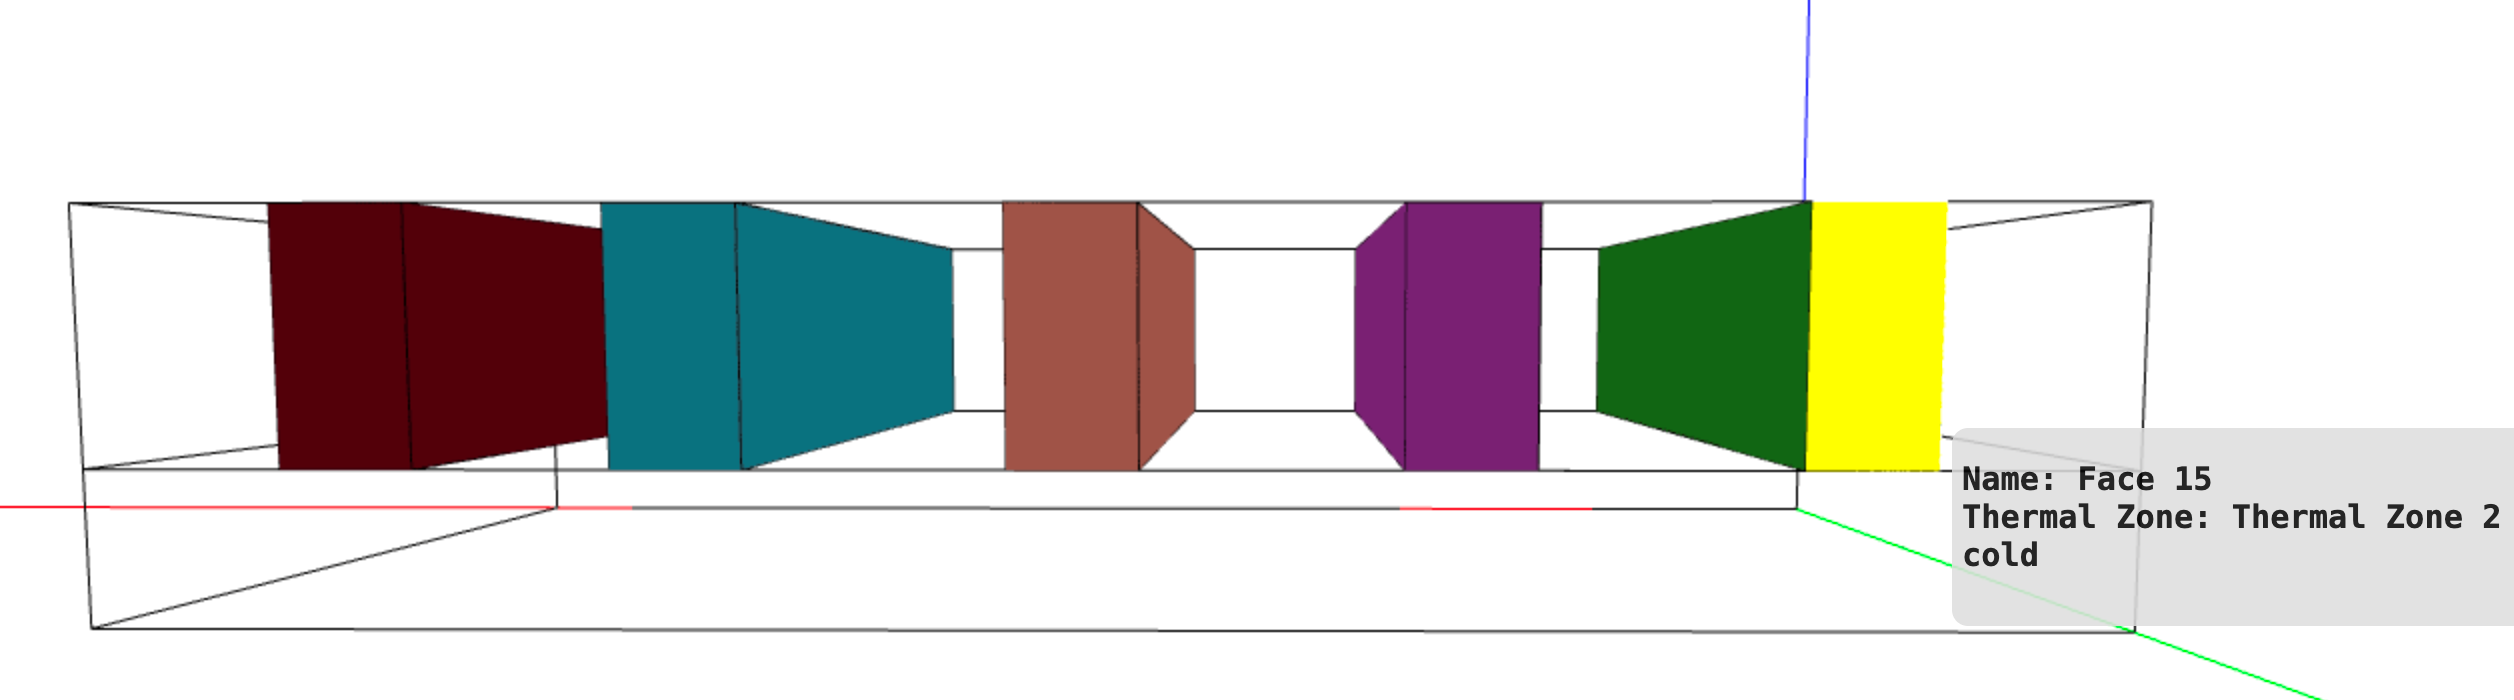
\includegraphics[width=0.95\linewidth]{figures/aisles_zones.png}
\caption{Холодные коридоры в модели ЦОД.}
\label{fig:aisles_zones}
\end{figure}

Компонентная визуализация системы CRAH представлена на Рис \ref{fig:CRAH1}. Воздух, попадающий в систему (в том числе наружный), проходит через змеевик водяного охлаждения (CRAH Water Cooling Coil), который охлаждается в Chilled Water Loop (Рис. \ref{fig:CRAH2}) (внутри него используется Condenser Water Loop (Рис. \ref{fig:CRAH3})). После происходит контроль влажности воздуха, и воздух через CRAH Fan, попадает в фальшпол, в VAV Terminal, а затем в холодные коридоры.

\begin{figure}[h!]
\centering
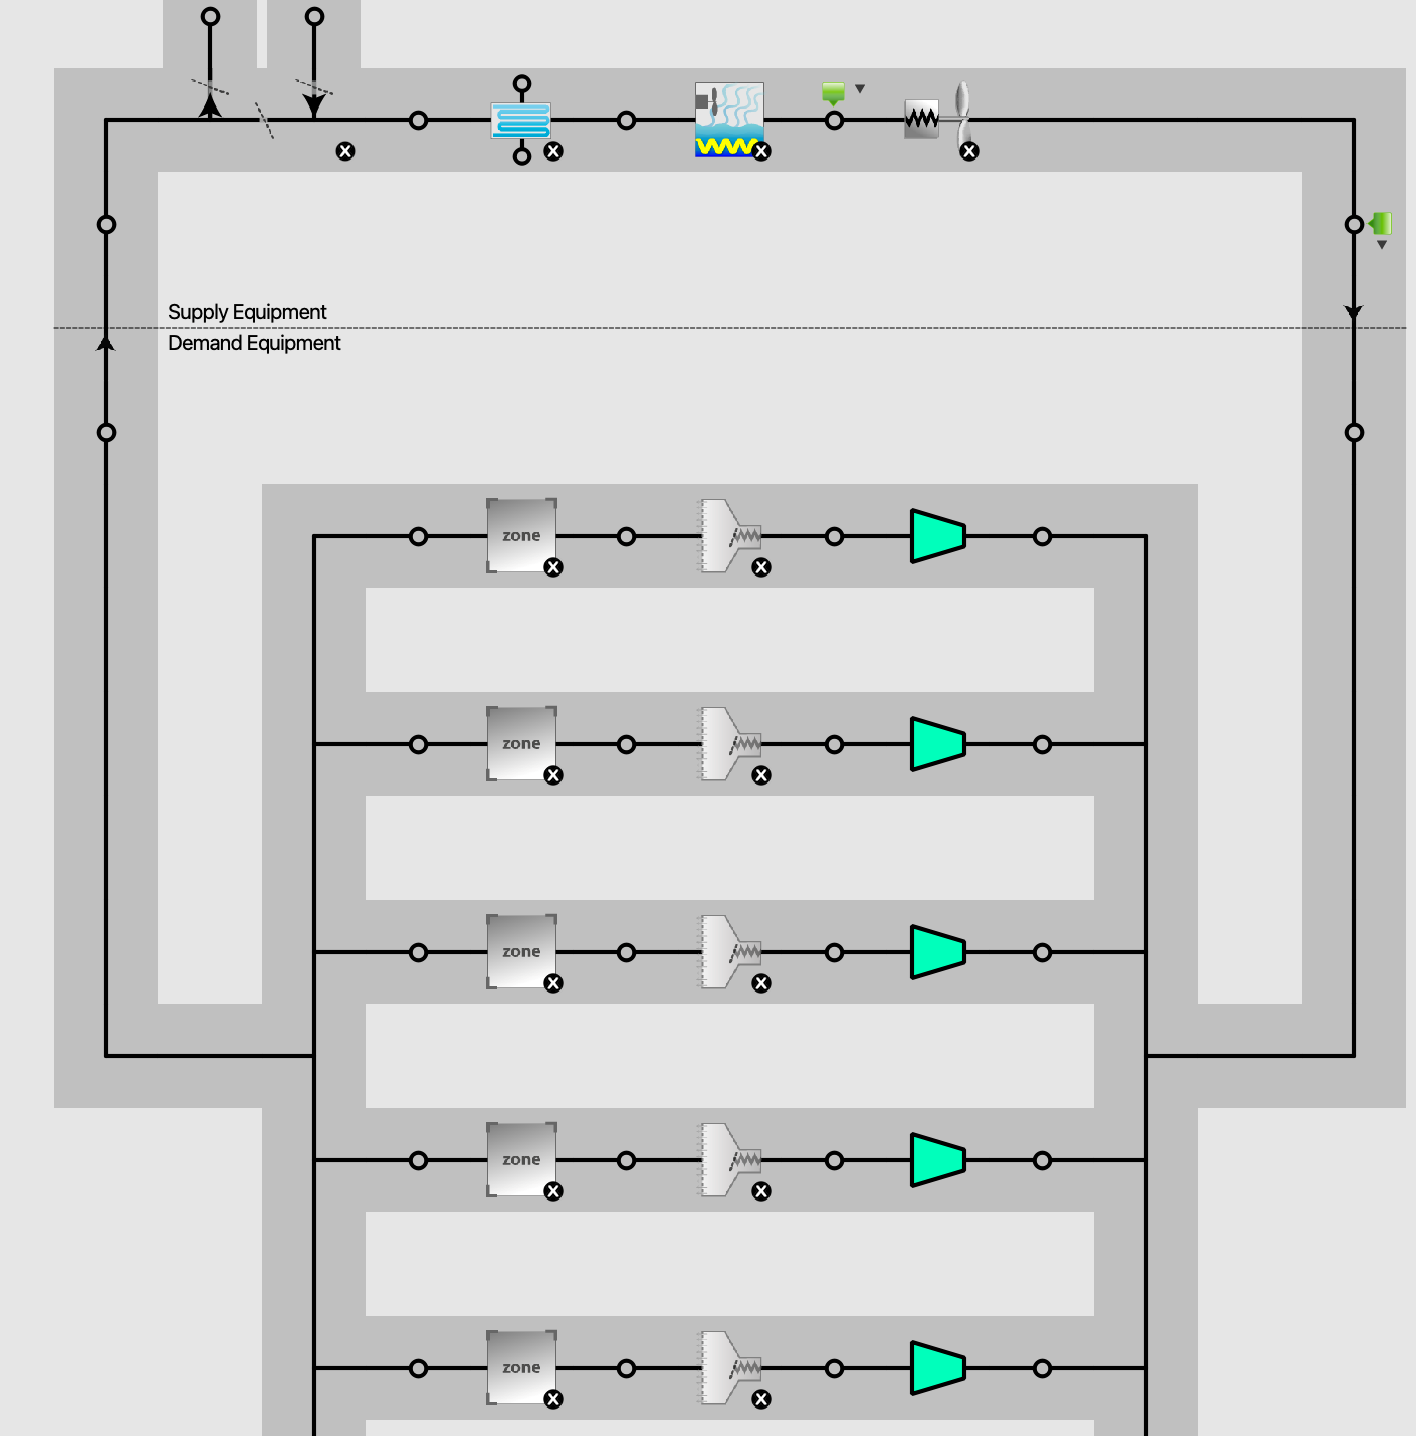
\includegraphics[width=0.95\linewidth]{figures/CRAH1.png}
\caption{Компоненты системы CRAH.}
\label{fig:CRAH1}
\end{figure}

\begin{figure}[h!]
\centering
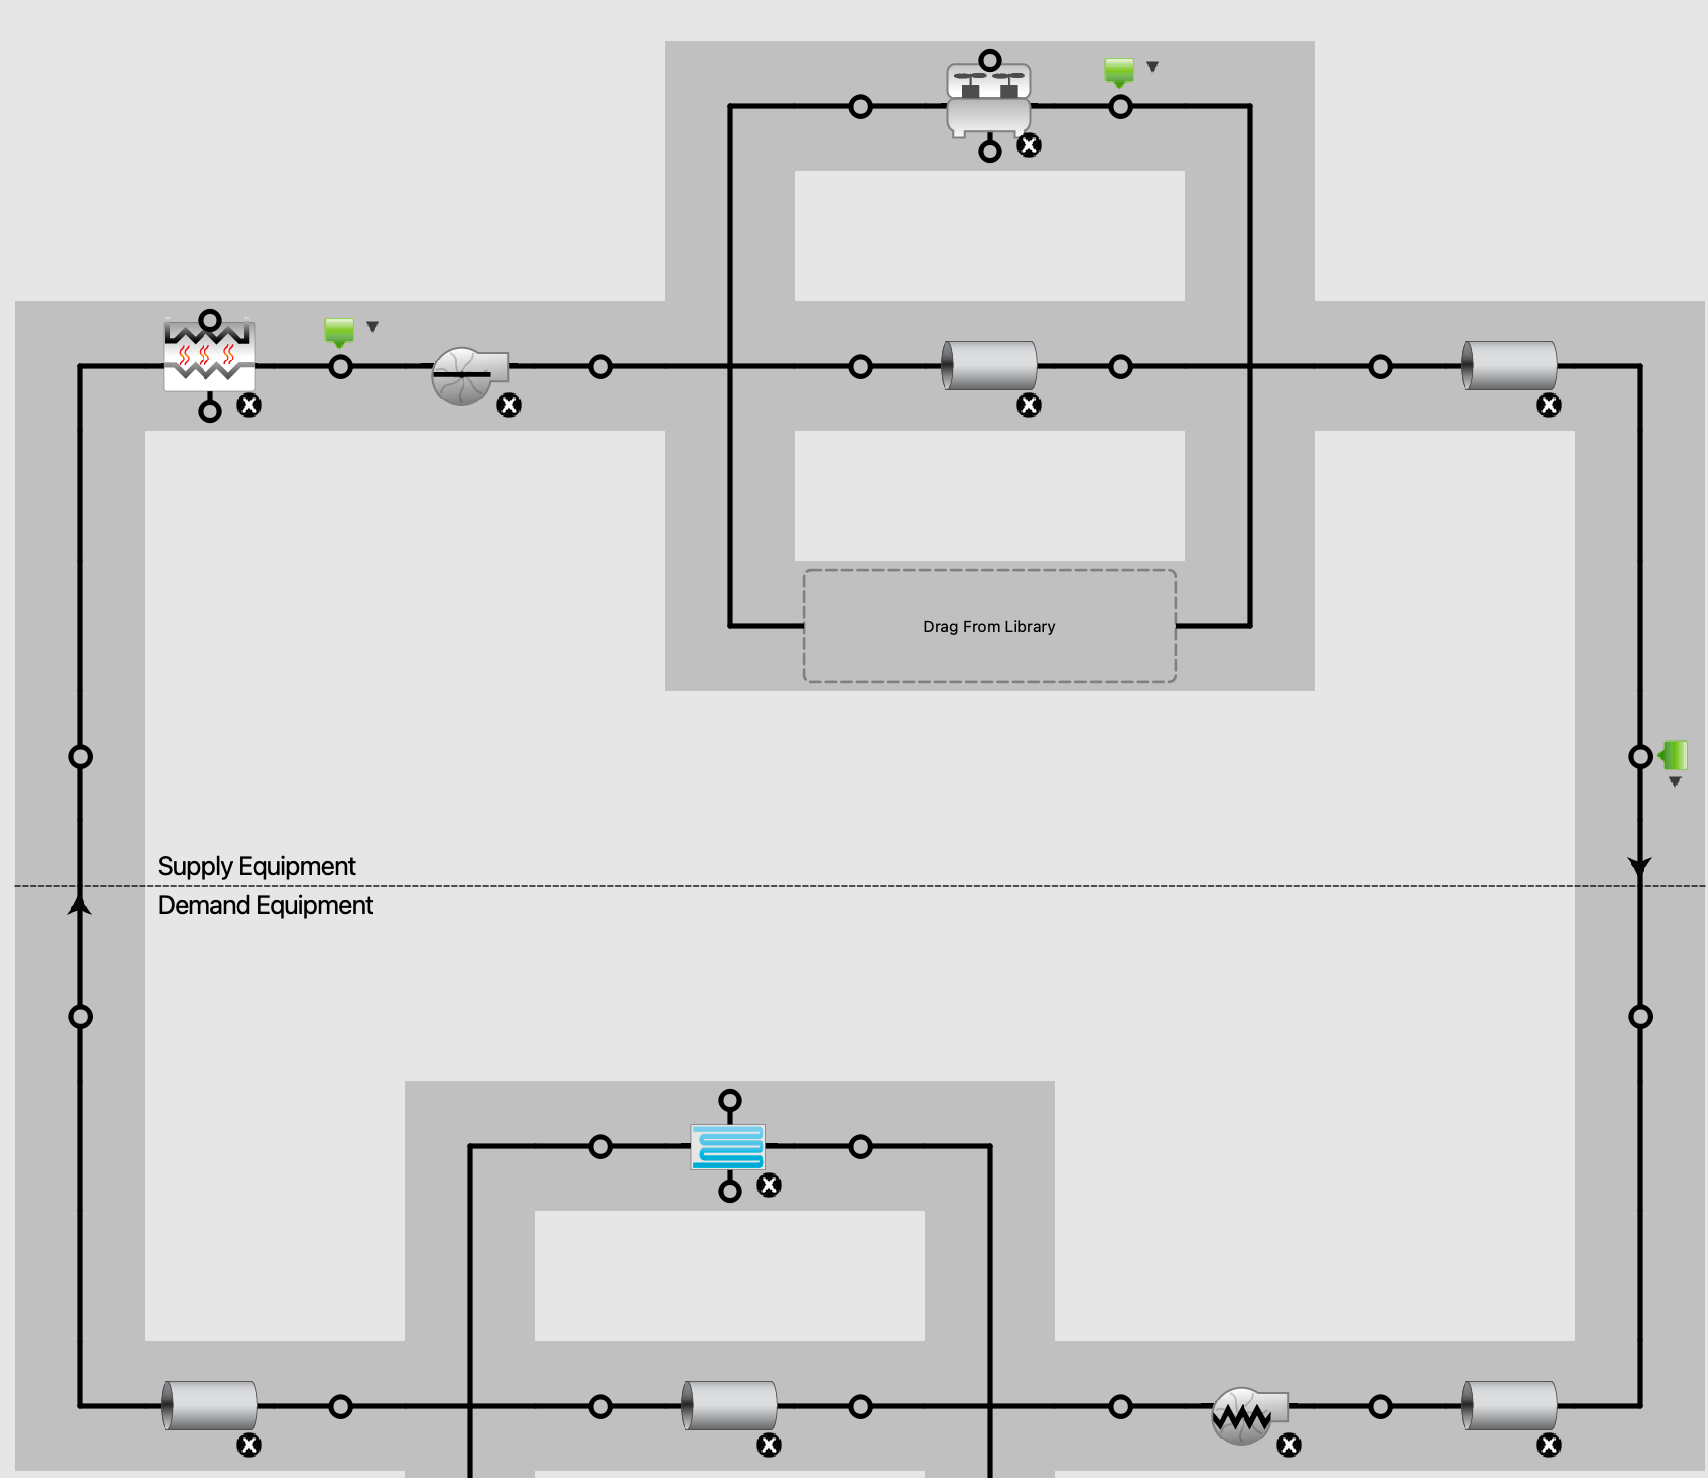
\includegraphics[width=0.95\linewidth]{figures/CRAH2.png}
\caption{Компоненты системы Chilled Water Loop.}
\label{fig:CRAH2}
\end{figure}

\begin{figure}[h!]
\centering
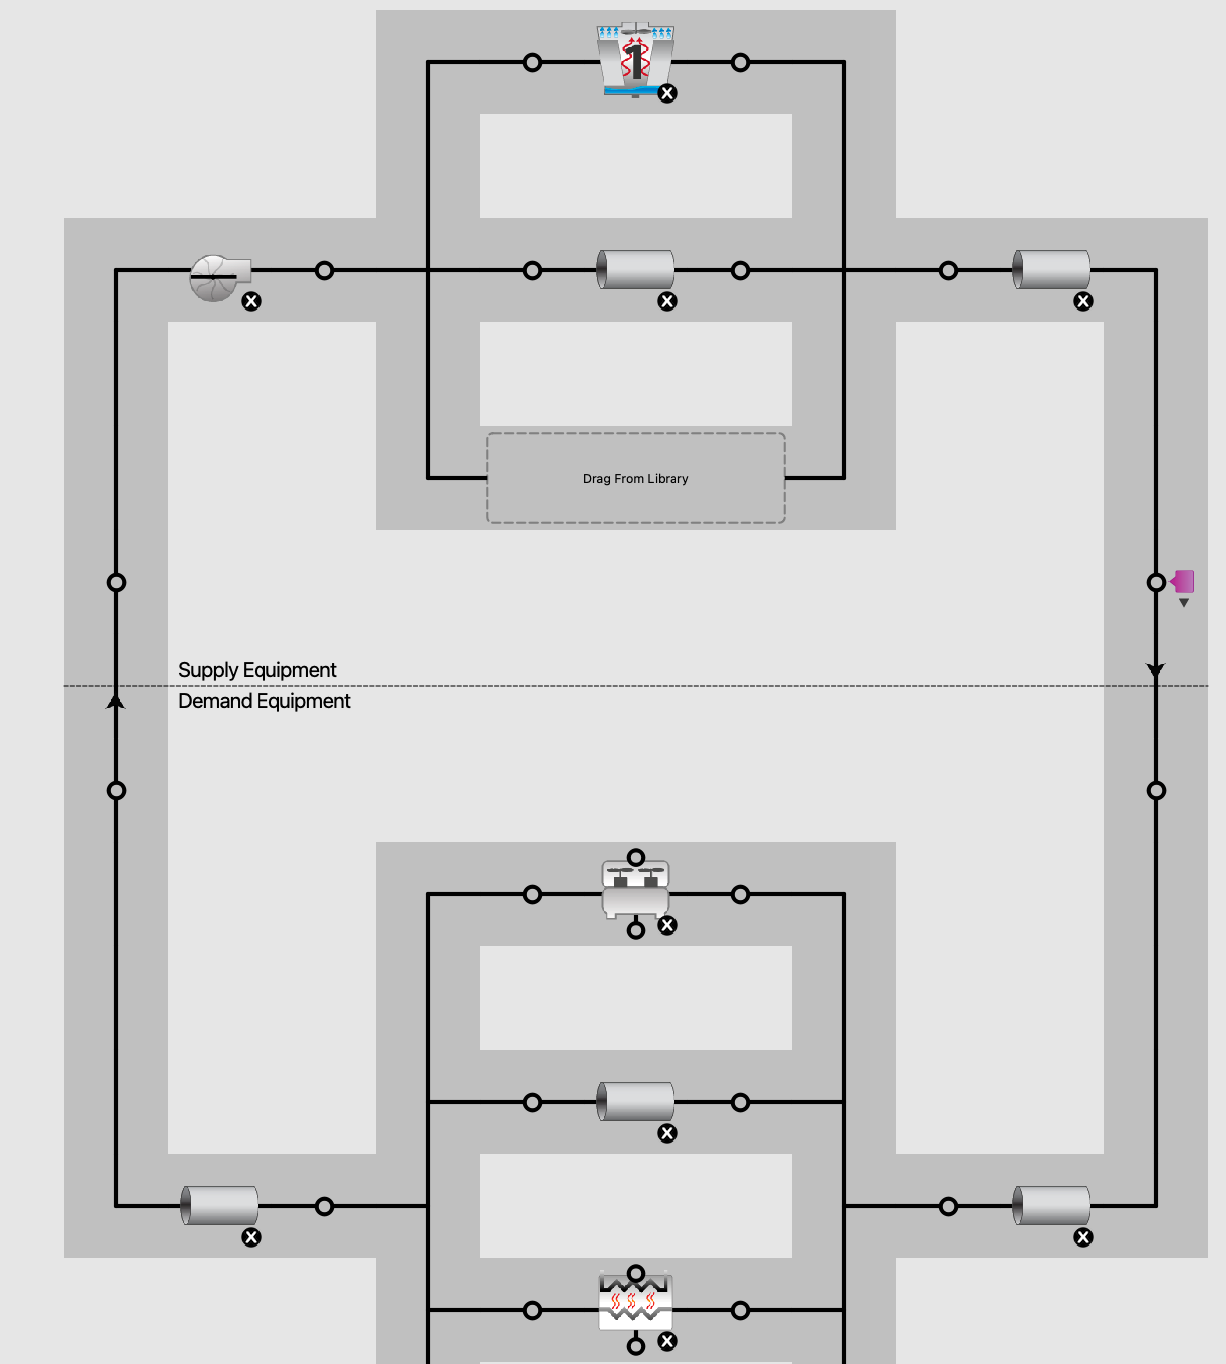
\includegraphics[width=0.95\linewidth]{figures/CRAH3.png}
\caption{Компоненты системы Condenser Water Loop.}
\label{fig:CRAH3}
\end{figure}

Для каждого компонента каждой системы подобраны параметры.

В модель добавлены данные о погоде в Москве из источников ASHRAE \href{https://energyplus.net/weather-location/europe_wmo_region_6/RUS/RUS_Moscow.276120_IWEC }{(ссылка)}, информация о уровне CO\textsubscript{2}, информация о осветительной нагрузке и другое.

Далее модель дорабатывалсь уже в самом файле с кодом описания модели.

Это очень общее описание модели, каждый компонент настраивался отдельно, полное описание модели на языке разметики, который читает EnergyPlus, представлен \href{https://github.com/koshachya-myata/Data_Center_Simulation/blob/main/src/dc_env/buildings/MultiZone_DC_wHot_nCold_Aisles/MultiZone_DC.idf}{здесь}.

\subsection{Взаимодействие с Python и RL-агентом}
Необходимо было добавить возможность влиять на симуляцию в процессе исполнения (чтобы RL-агент мог управлять уставками). Для этого применялись ExternalInterface на расписаниях (Schedule) управляемых объектов, управление ими проводилось посредством Ptolemy2 и Building Controls Virtual Test Bed (\href{https://github.com/lbl-srg/bcvtb }{bctvb}). Передача и получение информации от процесса EnergyPlus велось поверх сокетов.

\section{Получение RL-агента}

\subsection{Среда для обучения}
Создавалась среда ЦОД, в которой RL-агент может делать шаги, получать награду и т.п. Среда напрямую давала агенту возможность взаимодействовала с моделю ЦОД, описанной выше, запускала ее симуляцию, совершала действия агента, получала информацию на основе которой строила награждение. Среда наследовала базовый класс среды от \href{https://gymnasium.farama.org/index.html}{gymnasium}. В коде описан как и общий абстрактный класс для всех сред ЦОД, так и конкретный для среды, которая взаимодействует с EnergyPlus. Более полно можно посмотреть в \href{https://github.com/koshachya-myata/Data_Center_Simulation/blob/main/src/dc_env/data_center_env.py}{исходном коде}, в нем описаны докстринги и типизация каждого метода.

\subsection{Обучение агента}
Проводилось много экспериментов, обучались агенты с помощью Ray и stable baselines 3 (SB3). Исследовались модели PPO, A2C, SAC. Сейчас как модель для теста инференса стоит PPO от SB3, которая обучалась с использованием transfer learning, сначала модель обучалась в симуляции на 1 день, потом на 3 и тд, также в процессе обучения изменялся learning rate. Большая проблема заключалась в том, что модели обучается достаточно долго, и большое время занимает один шаг агента. Так, SAC обучался более устойчиво, но одна эпоха длилась в 2 раза больше, чем у PPO, поэтому модель SAC не очень подходила для обучения бейзлайн модели на одном процессоре. Из-за этого таже сокращена размерность observation space агента, он видит не всю информацию о зонах, а только информацию о температурах в крайних и центральном коридорах, влажность в центральной зоне, наружную температуру воздуха, и предыдущие уставки охлаждения и температуры воздуха AHU (эксперименты показали, что если агенту поступает информация о предыдущих уставках, то он обучается лучше). Также в процессе обучения стало ясно, что агент лучше обучается, если он принимает от среды и отдает ей нормализованные числа.

\subsection{Сравнение агента и костантных моделей}
Сравнение данных симуляции при контроле уставок RL-агентом оказалось эффективнее, чем при контроле константными уставками. Наглядно это можно посмотреть в  \href{https://github.com/koshachya-myata/Data_Center_Simulation/blob/main/notebooks/statistics.ipynb}{ноутбуке}.

\subsection{HTTP-API}
С использованием Flask построена HTTP-API для RL-агента. Запускается сервер, который отлавливает json'ы приходящие на POST запрос в в \Verb+/predict+, из json берется список наблюдений (observations), который подается в модель. Модель возвращает набор действий; действия добавляется в json, который возвращается клиенту.

\section{Логирование и дэшборды}
Добавлен код для создания и заполнения БД и таблицы ClickHouse. Добавлен архив с дэшбордом Superset.

Также добавлена возжность сделать симуляцию инференса: запустить http-API, запустить среду ЦОД, каждый шаг которой отправляется с использованием API, создать таблицу ClickHouse и каждый шаг добавлять туда информацию от среды.

\section{Описание структуры проекта}

Ниже описаны самые важные компоненты структуры проекта.

\Verb+main.py+ управляет запуском главных функций.

\Verb+Makefile+ вызывает \Verb+main.py+ с нужными аргументами в более user-friendly виде, а также имеет различные удобные правила.

\Verb+config.py+ позволяет указать путь до EnergyPlus и настроить ожидаемый процесс симуляции в коде (нужно, чтобы он соответствовал параметрам в \Verb+.idf+ файле).

\Verb+data/+ хранит parquet файлы, полученные в результате тестирования агента и константных моделей.

\Verb+models/+ хранит предобученные модели.

\Verb+notebooks/+ хранит ноутбук с сравнением агента и константных моделей.

\Verb+external/DC_dashboard+ -- дэшборд для Superset.

\Verb+src/+ весь основной код.

\Verb+src/eplus_controll/+ весь необходимый функционал для работы с EnergyPlus.

\Verb+src/dc_env/buildings/MultiZone_DC.idf+ хранит описание модели ЦОД

\Verb+src/dc_env/data_center_env.py+ хранит класс среды для ЦОД.

\Verb+src/models/+ весь функционал для обучения и теста модели (внутри разделение на константные модели, модели из Ray и модели из SB3).

\Verb+src/inference/model_api.py+ описание HTTP-API агента.

\Verb+src/inference/DBApi.py+ класс дя взаимодействия с ClickHouse.

\Verb+src/inference/inference_agent.py+ для симуляции инференса RL-агента.

\end{document}